\documentclass{uetgraduation}
\graphicspath{{graph/}}
\begin{document}
\studentname{Hoàng Trung Dũng}
\title{Nghiên cứu phương pháp chống nhiễu cho mạng truyền thông tán xạ ngược sử dụng phương pháp học sâu tăng cường}
\documenttype{Đồ án tốt nghiệp đại học hệ chính quy}
\major{Công nghệ thông tin}
\year{2024}
\supervisor{TS. Nguyễn Ngọc Tân}
\makecovers
% Tóm tắt
\begin{preamble}{Tóm tắt}
\textbf{Tóm tắt:} Truyền thông không dây đã và đang đóng vai trò vô cùng quan trọng trong cuộc sống con người. Tuy
nhiên phương pháp truyền thông này lại rất dễ bị tấn công gây nhiễu do tín hiệu vô tuyến phát sóng trong không gian mở.
Thêm vào đó, với sự phát triển của UAV (thiết bị bay không người lái) với khả năng cung cấp đường truyền tầm nhìn thẳng
(LoS) và hệ số suy giảm đường truyền thấp đã hỗ trợ cho việc tấn công đối với kết nối không dây. Trong khoá luận tốt nghiệp
này, em muốn trình bày một phương án chống nhiễu cho mạng truyền thông không dây, sử dụng học tăng cường sâu, kết hợp với
kỹ thuật tán xạ ngược và thu hoạch năng lượng để không những chống lại mà còn tận dụng được tín hiệu gây nhiễu từ UAV 
để nâng cao hiệu suất của hệ thống truyền thông không dây.

\textit{\textbf{Từ khóa:} Truyền thông không dây, Nhiễu, UAV, Học tăng cường sâu, Tán xạ ngược, Thu năng lượng.}
\end{preamble}
% Lời cảm ơn
\begin{preamble}{Lời cảm ơn}
    Đầu tiên, cho phép em gửi lời cảm ơn đến các thầy, cô giáo trường Đại học Công nghệ - Đại học
    Quốc Gia Hà Nội đã luôn tận tình chỉ bảo và tạo điều kiện trong suốt quá trình em học
    tập tại trường.
    
    Em xin gửi lời cảm ơn sâu sắc đến thầy giáo TS. Nguyễn Ngọc Tân đã tận tình
    hướng dẫn và đóng góp ý kiến quý báu trong suốt quá trình thực hiện khóa luận tốt
    nghiệp của em.
    
    Cuối cùng em xin gửi lời cảm ơn đến gia đình của mình, nơi đã luôn là nguồn động lực cho em
    trong suốt thời gian vừa qua.
    
    Em xin chân thành cảm ơn.
\end{preamble}
% Lời cam đoan
\begin{preamble}{Lời cam đoan}
Tôi xin cam đoan rằng mọi kết quả trình bày trong khóa luận đều do tôi thực hiện
dưới sự hướng dẫn của TS. Nguyễn Ngọc Tân.

Tất cả các tham khảo nghiên cứu liên quan đều nêu rõ nguồn gốc một cách rõ ràng từ 
danh mục tài liệu tham khảo trong khóa luận. Khóa luận không sao chép tài liệu, 
công trình nghiên cứu từ người khác mà không có rõ về mặt tài liệu tham khảo.

Các thông kê, các kết quả trình bày khóa luận đều là tự thực nghiệm khi chạy chương trình. Nếu tôi sai 
tôi hoàn toàn chịu trách nhiệm theo quy định của trường Đại học Công Nghệ - Đại học Quốc Gia Hà Nội.

\begin{flushright}
    Hà Nội, tháng 12 năm 2024

    \vspace{45pt}
    Hoàng Trung Dũng
\end{flushright}
\end{preamble}

% Muc luc
\begin{contentlisting}

\tableofcontents
\listoffigures
% \listoftables

\begin{contentlistingsection}{Các từ viết tắt}
    UAV: unmanned aerial vehicle -- Thiết bị bay không người lái

    LoS: line-of-sight -- Đường truyền tầm nhìn thẳng

    RL: reinforcement learning -- Học tăng cường

    DRL: deep reinforcement learning -- Học tăng cường sâu.
    
    DQN: deep q network -- Mạng sâu Q.

    HTT: harvest then transmit -- Chiến lược thu năng lượng để truyền tin

    RA: rate adaption -- Kĩ thuật điều chỉnh tốc độ phát gói tin

    PSR: packet send ratio -- Tỉ lệ gói tin được máy phát gửi

    PDR: packet delivery ratio -- Tỉ lệ gói tin được gửi thành công đến máy thu

    MAC: medium access control -- Điều khiển truy nhập môi trường

    WLAN: wireless local area network -- Mạng cục bộ không dây

    WSN: wireless sensor network -- Mạng cảm biến không dây

    FHSS: frequency hopping spread spectrum -- Trải phổ nhảy tần

    RA: rate adaption -- Điều chỉnh tốc độ

    RFID: radio frequency identification -- Nhận dạng tần số vô tuyến

    ATG: air-to-ground -- Kênh truyền không đối đất

    MDP: Markov decision process -- Quá trình ra quyết định Markov
\end{contentlistingsection}

\end{contentlisting}

% Chapter 1
\chapter{Đặt vấn đề}
Truyền thông không dây là thành phần không thể thiếu trong cơ sở hạ tầng viễn thông của xã hội ngày nay, có các ứng dụng và
tác động sâu rộng đến mọi mặt của đời sống con người. Mặc dù công nghệ truyền thông không dây đã có rất nhiều bước phát triển
qua nhiều thập kỉ, hầu hết các mạng truyền thông không dây vẫn dễ bị tấn công gây nhiễu bởi tính mở của nó. Bằng cách đưa tín
hiệu nhiễu vào kênh không dây đích, thiết bị gây nhiễu có thể làm giảm tỉ lệ tín hiệu trên nhiễu cộng nhiễu (SINR) của máy thu,
qua đó làm gián đoạn hoặc ngăn chặn kênh truyền không dây hợp lệ. Không giống như những tác động không có chủ đích, tín hiệu gây
nhiễu thường mạnh và qua đó có thể liên tục làm gián đoạn kênh truyền.

Gần đây, thiết bị bay không người lái (UAV) đang ngày càng được sử dụng nhiều hơn để nâng cao năng lực của hạ tầng mạng. Khả năng
triển khai nhanh cùng với tính cơ động cao của UAV khiến nó phù hợp với rất nhiều nhiệm vụ, ví dụ như việc triển khai hệ thống
mạng tạm thời ở những nơi khó tiếp cận như những vùng xảy ra thiên tai, bão lũ... UAV có thể cung cấp đường truyền LoS và hệ số suy
giảm kênh truyền thấp đến người dùng trên mặt đất khi nó được sử dụng như một trạm phát sóng. Do đó UAV có thể được sử dụng để
tăng cường năng lực của hệ thống mạng. Tuy nhiên chính những lợi thế của UAV như ở trên khiến cho nó có thể bị đối tượng xấu 
khai thác như là một thiết bị gây nhiễu di động, ngăn chặn đáng kể việc truyền dữ liệu và làm giảm chất lượng dịch vụ (QoS) của mạng
không dây, nghiêm trọng hơn so với gây nhiễu từ trên mặt đất. Vì thế giải quyết vấn đề gây nhiễu từ UAV là một bài toán đáng quan tâm.

Trong khoá luận này, em sẽ tìm hiểu về tấn công gây nhiễu, cũng như tấn công gây nhiễu từ UAV đối với mạng truyền thông không dây.
Qua đó đề xuất một phương án để không những chống lại mà còn tận dụng cuộc tấn công gây nhiễu để đảm bảo chất lượng đường truyền.
Phần còn lại của khoá luận sẽ được chia thành các chương với nội dung cụ thể như sau:

Chương 2: Cơ sở lý thuyết. Trong chương này trình bày lý thuyết nền tảng về tấn công gây nhiễu và tấn công gây nhiễu bằng UAV.
Cũng như tìm hiểu một số chiến lược chống nhiễu đã được nghiên cứu. Sau đó sẽ đi vào tìm hiểu về RL và DRL - hai phương pháp được
sử dụng để chống nhiễu.

Chương 3: Đề xuất phương án giải quyết bài toán tấn công gây nhiễu từ UAV. Trong chương này, em sẽ mô hình hoá bài toán tấn công
gây nhiễu bằng UAV và đề xuất phương pháp chống nhiễu sử dụng DRL.

Chương 4: Thiết lập mô phỏng và kết quả mô phỏng. Trong chương này, em sẽ trình bày chi tiết về mô hình và thông số thiết lập mô
phỏng phương pháp chống nhiễu được đề xuất. Cũng như so sánh hiệu quả mà phương pháp đề xuất mang lại so với chiến lược phòng thủ
''tham lam''.

Chương 5: Kết luận.

% Chapter 2
\chapter{Cơ sở lý thuyết.}
\section{Mạng không dây.}
\subsection{Giới thiệu.}
Mạng không dây là một hệ thống mạng truyền tải dữ liệu mà không sử dụng các dây cáp kết nối vật lý. Thay vào đó, mạng không dây sử dụng sóng
điện từ để truyền tín hiệu và dữ liệu giữa các thiết bị. Điều này giúp tăng tính di động của thiết bị, vốn là điểm yếu của các kết nối của các
kết nối có dây. Phương pháp gửi dữ liệu thông qua môi trường không khí này được ứng dụng vô cùng sâu rộng trong mọi lĩnh vực đời sống con người
ngày nay, từ công sở, trường học hoặc thậm chí là trong quân sự\dots

Dữ liệu nhận và gửi của mạng không dây được truyền đi xuyên suốt thông qua các tầng ảo sau:
\begin{itemize}
    \item Tầng vật lý: Là tầng thể hiện đặc điểm của kết nối vật lý giữa các thiết bị trong mạng, trong trường hợp mạng không dây, môi trường truyền
    là không khí. Quá trình nhận và truyền dữ liệu được quản lý bởi tầng vật lý. Trong mạng không dây, dữ liệu nhị phân giữa các thiết bị được chuyển
    thành tín hiệu điện và sử dụng tần số vô tuyến để gửi và nhận dữ liệu, tất cả quá trình này được thực hiện bởi tầng vật lý. Đây cũng là tầng chịu
    thiệt hại nặng nề nhất từ cuộc tấn công gây nhiễu sóng vô tuyến.
    \item Tầng liên kết dữ liệu: Là tầng ở giữa, chịu trách nhiệm kết nối giữa tầng vật lý và tầng mạng, ngoài ra còn thực hiện phân đoạn các gói được
    gửi bởi các tầng cao hơn thành các khung có thể được gửi bởi tầng vật lý. Tầng này cũng cung cấp khả năng kiểm tra lỗi và định dạng các khung dữ liệu
    được gửi. Tầng con MAC của tầng liên kết dữ liệu chịu trách nhiệm di chuyển các gói dữ liệu đến và đi từ nút này sang nút khác trên một kênh chung.
    Kênh truyền trong mạng không dây là một tần số mà các nút sử dụng để gửi dữ liệu. Tầng con MAC sử dụng giao thức MAC để đảm bảo tín hiệu gửi từ các
    trạm khác nhau trên cùng một kênh truyền không bị xung đột. Tầng này dễ bị tấn công gây nhiễu tầng liên kết dữ liệu - các thiết bị gây nhiễu tinh vi
    có thể tận dụng lợi thế của tầng liên kết dữ liệu và tạo ra cuộc tấn công hiệu quả về mặt năng lượng. So với tấn công gây nhiễu sóng vô tuyến ở tầng
    vật lý, gây nhiễu tầng liên kết dữ liệu tối ưu hơn về mặt năng lượng.
    \item Tầng mạng: Hoạt động như một liên kết giữa tầng giao vận ở trên và tầng liên kết dữ liệu ở dưới. Chịu trách nhiệm tìm ra cấu trúc mạng và gán địa
    chỉ, cũng như định tuyến dữ liệu.
    \item Tầng giao vận: Khôi phục dữ liệu bị mất và cũng chịu trách nhiệm truyền lại dữ liệu. Cung cấp khả năng mã hoá dữ liệu và truyền dữ liệu đáng tin cậy.
    \item Tầng ứng dụng: Tầng này chịu trách nhiệm xác định thông số kỹ thuật của dữ liệu được yêu cầu bởi cả người dùng cuối cũng như các nút trong mạng. 
\end{itemize}

\subsection{Phân loại mạng không dây và ứng dụng.}
\begin{itemize}
    \item WLAN: mạng không dây cục bộ, hay còn được biết đến nhiều hơn là Wi-Fi. WLAN cho phép thiết bị kết nối với Internet dễ dàng miễn là nó được kết nối với
    sóng Wi-Fi. WLAN được sử dụng ở rất nhiều nơi xung quanh chúng ta ngày nay, từ hộ gia đình, trường học, công sở, địa điểm kinh doanh\dots Thiết bị di động
    kết nối với điểm truy cập thông qua kết nối không dây sẽ có thể kết nối Internet và di chuyển một cách tự do, miễn là thiết bị đó ở trong tầm phủ sóng của
    sóng Wi-Fi.

    Hình 2.1 mô tả một mạng không dây cục bộ với một điểm truy cập và bốn thiết bị kết nối thông qua môi trường không dây.
    \begin{figure}{Mạng không dây cục bộ.}
        \centering
        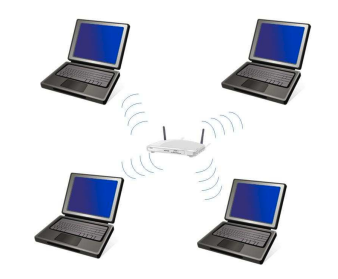
\includegraphics[scale=0.6]{wlan}
        \label{fig:wlan}
    \end{figure}
    \item WSN: Mạng cảm biến không dây, là một tập hợp số lượng lớn các nút có khả năng thu thập dữ liệu từ môi trường xung quanh và truyền tải thông tin
    về trung tâm xử lý dữ liệu hoặc các thiết bị thu thập dữ liệu. Trong WSN, các nút có thể chia sẻ thông tin cho nhau, dữ liệu thu thập từ các cảm biến không được
    gửi trực tiếp cho người dùng mà được xử lý và tổng hợp lại, chỉ gửi những thông tin mục tiêu mà mạng cảm biến muốn đạt được. Do đó những dữ liệu tạm thời, không
    cần thiết, chưa qua xử lý hoặc dữ liệu trung gian giữa các nút sẽ không được gửi tới người dùng.
    \begin{figure}{Mạng cảm biến không dây.}
        \centering
        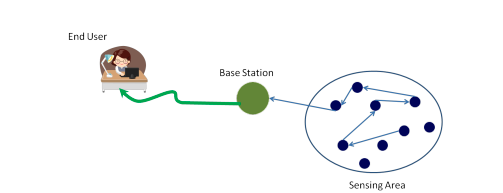
\includegraphics[scale=0.6]{wsn}
        \label{fig:wsn}
    \end{figure}

    Mạng cảm biến không dây có một số ứng dụng sau:
    \begin{itemize}
        \item Sử dụng trong lĩnh vực an ninh như giám sát ở các khu vực nhạy cảm để phát hiện các mối đe doạ như tấn công sinh học hoặc hoá học\dots
        \item Giám sát môi trường: WSN hỗ trợ thu thập thông tin ở những khu vực khó thiết lập cơ sở hạ tầng để giám sát môi trường cũng như môi trường sống.
        \item Trong y học: sử dụng để giúp các bác sĩ theo dõi sức khoẻ của bệnh nhân.
        \item Theo dõi đối tượng: WSN có thể dùng để theo dõi các đối tượng chuyển động nếu sử dụng cảm biến phù hợp.
        \item Hỗ trợ người khuyết tật: Người khuyết tật có thể độc lập hơn và cải thiện khả năng hoạt động với việc sử dụng WSN, WSN cho phép tự chăm sóc hiệu
        quả hơn và nâng cao chất lượng cuộc sống.
    \end{itemize}

    \item Mạng không dây tạm thời (ad hoc): là mạng không dây không cần bất kì cơ sở hạ tầng hiện có nào để triển khai ví dụ như điểm truy cập hoặc dây cáp.
    Mỗi thiết bị trong mạng coi là một nút tham gia trực tiếp vào việc định tuyến dữ liệu một cách độc lập bằng cách chuyển tiếp dữ liệu từ nút này sang nút khác
    mà không cần thêm bất kì một thiết bị quản lý tập trung nào như điểm truy cập\dots Mỗi nút trong mạng không dây tạm thời tự động quyết định nút nào sẽ gửi dữ
    liệu tiếp theo tuỳ thuộc vào kết nối mạng. Hình 2.3 là một mô hình đơn giản của mạng không dây tạm thời giữa các thiết bị kết nối với nhau mà không có điểm
    truy cập nào.
    \begin{figure}{Mạng không dây tạm thời.}
        \centering
        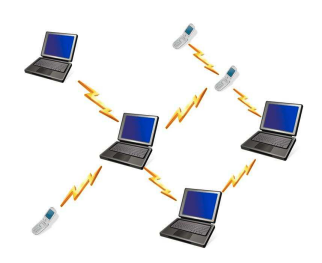
\includegraphics[scale=0.6]{ad_hoc}
        \label{fig:adhoc}
    \end{figure}

    Ứng dụng của mạng không dây tạm thời:
    \begin{itemize}
        \item Trong quân sự: người lính, các thiết bị quân sự như xe tăng, tàu chiến có thể kết nối với nhau mà không cần một cơ sở hạ tầng mạng không dây rõ ràng
        bằng cách hình thành một mạng không dây tạm thời.
        \item Mạng không dây tạm thời có thể được sử dụng trong các nhiệm vụ thực thi pháp luật, giải cứu\dots
        \item Có thể được sử dụng trong hội nghị, cuộc họp, bài giảng hoặc các khu vực phục vụ mục đích thương mại, nơi tải mạng có thể rất cao.
    \end{itemize}
\end{itemize}


\section{Tấn công gây nhiễu sóng vô tuyến.}
Trong mạng truyền thông không dây, đặc tính mở của môi trường truyền, cụ thể ở đây mạng không dây sử dụng không khí là môi trường truyền để truyền và nhận dữ
liệu, dẫn đến việc nó rất dễ bị tấn công bởi nhiều kiểu tấn công khác nhau. Ở đây chúng ta nghiên cứu cụ thể loại tấn công mạng không dây bằng gây nhiễu sóng
vô tuyến.

\subsection{Giới thiệu.}
Tấn công gây nhiễu sóng vô tuyến được định nghĩa là một hành động cố tình can thiệp vào quá trình truyền và nhận vật lý của truyền thông
không dây. Trong đó kẻ tấn công (máy gây nhiễu) sẽ phát tín hiệu vô tuyến trên cùng băng tần mà mạng mục tiêu sử dụng. Mục tiêu của việc
tấn công là làm giảm hiệu suất mạng hoặc thậm chí ngăn chặn hoàn toàn việc truyền thông tin không dây giữa các thiết bị.

Trong cuộc tấn công gây nhiễu, máy gây nhiễu đưa năng lượng gây nhiễu vào môi trường không dây, gây cản trở việc truyền tải hợp pháp theo
một trong hai cách: 
\begin{itemize}
    \item Máy gây nhiễu gửi tín hiệu nhiễu mạnh gây giảm tỉ lệ tín hiệu trên nhiễu cộng với nhiễu (SINR) ở máy thu.
    \item Gây nhiễu liên tục ngăn cản việc máy phát truy cập vào kênh truyền, dẫn đến một cuộc tấn công từ chối dịch vụ (DOS). Tấn công từ
    chối dịch vụ thực hiện bằng cách gửi tín hiệu nhiễu, gói tin giả khiến kênh truyền hợp lệ bận, làm cho máy phát ngừng gửi bất kì dữ liệu nào
    cho đến khi kênh truyền khả dụng trở lại.
\end{itemize}

Tấn công gây nhiễu sóng vô tuyến có một số đặc điểm sau đây:
\begin{itemize}
    \item Cố ý: Đây là hành động gây nhiễu có chủ đích của kẻ tấn công, nhằm vào một mục tiêu cụ thể, không giống với nhiễu tự nhiên gây
    ra bởi các yếu tố của môi trường.
    \item Không tuân thủ các giao thức MAC: đặc điểm chung của các cuộc tấn công gây nhiễu là việc liên lạc của chúng không tuân theo các
    giao thức MAC.
    \item Phạm vi tấn công: Máy gây nhiễu có thể nhắm vào một tần số cố định hoặc nhiều tần số khác nhau.
\end{itemize}

\subsection{Thông số đánh giá một cuộc tấn công gây nhiễu.}
Trong tấn công gây nhiễu sóng vô tuyến, các thông số sau phản ánh tác động của cuộc tấn công đến mạng không dây.
\begin{itemize}
    \item \textbf{SINR}: tỉ lệ tín hiệu trên nhiễu cộng nhiễu là tỉ số giữa công suất của tín hiệu máy phát so với tín hiệu gây nhiễu như
    tín hiệu từ máy gây nhiễu và nhiễu môi trường trong kênh truyền
    \[
    \theta = \frac{P_R}{\varphi P_J + \rho^2}
    \]
    Trong đó $P_R$ là công suất nhận được từ máy phát tại cổng (máy thu), $P_J$ là công suất nhiễu được phát của máy gây nhiễu, $\rho^2$ là phương sai
    của nhiễu Gauss trắng cộng thêm. $\varphi P_J$ là công suất nhiễu tại cổng, trong đó $0 \leq \varphi \leq 1$ là hệ số suy giảm kênh truyền.

    Có thể thấy tín hiệu nhiễu càng mạng càng làm giảm giá trị SINR ở máy thu, khiến cho tỉ lệ lỗi bit (BER) tăng, gây lỗi khi giải mã gói tin ở máy thu,
    làm giảm thông lượng và độ tin cậy của kết nối giữa máy phát và máy thu.
    \item \textbf{Thông lượng}: được định nghĩa là tốc độ trung bình gửi gói tin thành công thông qua kênh truyền, được tính thông qua công thức Shannon:
    \[
    C = B \log_2(1 + \text{SINR})
    \]
    Trong đó $C$ là dung lượng kênh hoặc thông lượng lý thuyết tối đa (bit/s), B là băng thông của kênh (Hz). Ta có thể nhận thấy thông qua công thức này,
    thông lượng của kênh giảm khi có sự xuất hiện của tín hiệu gây nhiễu làm giảm chỉ số SINR.
    \item \textbf{PSR}: đại diện cho tỉ lệ giữa gói tin thực sự được gửi thành công bởi máy phát và số gói tin mà máy phát dự định gửi. Nếu máy phát có ý
    định gửi n gói tin và máy thu chỉ nhận được m gói tin ($m \leq n$) thì PSR được tính như sau:
    \[
    PSR = \frac{m}{n}
    \]
    Số gói tin bị mất so với gói tin dự định gửi là do nhiễu. Tín hiệu nhiễu khiến cho kênh truyền luôn bận khiến máy phát không thể truyền gói tin đến máy
    thu, dẫn đến gói tin mới đến máy phát bị loại bỏ do hàng đợi gói tin của máy phát đầy, hoặc gói tin bị loại do ở quá lâu trong hàng đợi. Các giao thức
    MAC khác nhau có cách xác định kênh truyền đang bận hay không khác nhau, một trong số đó là nếu cường độ tín hiệu của kênh lớn hơn ngưỡng xác định trước,
    kênh sẽ được xác định là bận.
    \item \textbf{PDR}: là tỉ lệ số gói tin được gửi thành công đến máy thu so với số gói tin được máy phát gửi đi. Sau khi gói tin được máy phát gửi, máy thu
    vẫn có thể không giải mã được gói tin do ảnh hưởng của nhiễu, dẫn đến gói tin gửi không thành công. PDR có thể được tính ở máy thu bằng tỉ lệ giữa số gói
    tin nhận được và số gói tin vượt qua được kiểm tra CRC - là kĩ thuật phát hiện lỗi thường được dùng trong mạng truyền thông.
    
    Giả sử n là số gói tin máy thu nhận được và q là số gói tin vượt qua kiểm tra CRC thì:
    \[
    PDR = \frac{q}{n}
    \]
    Ngoài ra PDR còn có thể được tính ở máy phát bằng số gói tin ACK mà máy phát nhận được từ máy thu. Trong cả 2 trường hợp, nếu không có gói tin nào nhận thành
    công ở máy thu, PDR được xác định là 0.
\end{itemize}


\subsection{Các mô hình tấn công gây nhiễu.}
Có rất nhiều chiến lược tấn công khác nhau mà máy gây nhiễu có thể thực hiện để làm nhiễu mạng không dây. Do đó cũng dẫn đến nhiều mô hình tấn công với
nhiều mức độ hiệu quả khác nhau. Tuy nhiên sau đây là một số mô hình gây nhiễu đã chứng minh được tính hiệu quả trong việc làm gián đoạn kết nối mạng không
dây.
\begin{itemize}
    \item \textbf{Máy gây nhiễu liên tục}: thiết bị gây nhiễu liên tục phát ra tín hiệu vô tuyến mà không có sự gián đoạn. Tín hiệu nhiễu phát ra có thể 
    là sóng điện từ đơn giản hoặc thậm chí là các bit dữ liệu. Sóng điện từ hoặc các bit dữ liệu được máy gây nhiễu phát ra này không tuân theo bất kì giao 
    thức hoặc quy tắc nào mà các nút trong mạng tuân theo. Kiểu máy gây nhiễu này làm giảm PDR bằng cách làm hỏng các bit tại máy thu, khiến máy thu không
    thể giải mã dữ liệu. Nó cũng có thể làm giảm PSR bằng cách giữ cho kênh truyền giữa máy phát và máy thu liên tục bận, ngăn chặn việc máy phát truyền sử
    dụng đường truyền hợp lệ để truyền gói tin đến máy thu.
    \item \textbf{Máy gây nhiễu lừa đảo}: loại máy gây nhiễu này rất giống với máy gây nhiễu liên tục do cùng liên tục truyền tín hiệu hoặc dữ liệu qua mạng.
    Tuy nhiên điểm khác biệt là máy gây nhiễu lừa đảo không truyền các bit dữ liệu ngẫu nhiên. Máy gây nhiễu giả mạo liên tục đưa các gói tin vào mạng mà không
    có bất kì khoảng cách nào giữa các lần truyền, và do dữ liệu không phải là các bit ngẫu nhiên, do đó khiến cho nút mạng tin rằng những bit dữ liệu này là
    hợp lệ và do đó không sử dụng đường truyền nữa. Ví dụ máy gây nhiễu có thể gửi gói tin ACK giả mạo để khiến máy phát tin rằng nó đã truyền dữ liệu thành công.
    \item \textbf{Máy gây nhiễu ngẫu nhiên}: hai kiểu máy gây nhiễu ở trên luôn luôn duy trì việc truyền tín hiệu hoặc dữ liệu vào mạng, dẫn đến việc nó không
    hiệu quả về mặt năng lượng và phải kết nối với nguồn năng lượng bên ngoài khiến nó hạn chế khả năng di chuyển. Máy gây nhiễu ngẫu nhiên mặt khác có chu kỳ ngủ
    và chu kỳ gây nhiễu, cả hai chu kỳ có thể tuân theo một phân phối xác suất hoặc có thể hoàn toàn là ngẫu nhiên. Việc có cả hai trạng thái ngủ và gây nhiễu
    khiến máy gây nhiễu có thể tắt tín hiệu gây nhiễu qua đó tiết kiệm năng lượng trong giai đoạn ngủ và hoạt động như bất kỳ máy gây nhiễu nào trong hai máy gây 
    nhiễu đã thảo luận ở trên trong chu kỳ gây nhiễu của nó.
    \item \textbf{Máy gây nhiễu phản ứng}: ba mô hình gây nhiễu ở trên là ba mô hình gây nhiễu chủ động theo nghĩa là chúng luôn chủ động tấn công kênh truyền
    bất kể lưu lượng qua kênh như thế nào. Gây nhiễu chủ động thường hiệu quả vì chúng khiến kênh truyền luôn bận rộn, tuy nhiên lại có nhược điểm là dễ bị phát
    hiện. Một cách tiếp cận khác so với gây nhiễu chủ động là gây nhiễu phản ứng, tức là không cần thiết phải tấn công kênh truyền khi không có lưu lượng trên đường
    truyền. Thay vào đó máy gây nhiễu phản ứng sẽ không hoạt động khi kênh truyền rảnh rỗi, và bắt đầu phát tín hiệu gây nhiễu ngay khi nó cảm nhận được hoạt động
    truyền phát tín hiệu trên kênh. Do đó nó nhắm vào việc nhận tin nhắn. Thiết bị gây nhiễu phản ứng có thể không tối ưu về mặt năng lượng do nó phải liên tục lắng
    nghe để cảm nhận kênh truyền. Tuy nhiên nó khó bị phát hiện hơn gây nhiễu chủ động.
\end{itemize}

\section{Tấn công gây nhiễu bằng UAV.}
Trong phần này, chúng ta cùng xem xét về mô hình kênh truyền ATG giữa UAV và thiết bị trên mặt đất, qua đó đưa ra một số cơ sở lý thuyết về bài toán tấn công gây
nhiễu bằng UAV.

Xem xét một UAV gây nhiễu, thiết bị I nằm trên mặt đất chịu tác động của tín hiệu nhiễu UAV, kênh liên lạc giữa UAV và thiết bị I được mô 
hình hoá là kênh không đối đất ATG, bao gồm ba thành phần là:
\begin{itemize}
    \item Đường truyền tầm nhìn thẳng LoS: không có vật cản giữa UAV và thiết bị
    \item Đường truyền không tầm nhìn thẳng NLoS: tín hiệu không thể đi thẳng giữa UAV và thiết bị vì có vật cản như cây cối, toà nhà, địa hình\dots 
    \item Pha đinh quy mô nhỏ (small-scale fading): là sự biến động tín hiệu nhanh chóng do hiện tượng đa đường, gây ra các thay đổi về cường độ tín hiệu khi môi trường
    thay đổi\dots
\end{itemize}

Về cơ bản, tác động của pha đinh quy mô nhỏ nhỏ hơn nhiều so với LoS và NLoS, do đó yếu tố này bị bỏ qua. Suy hao đường truyền của kênh không đối đất giữa UAV và thiết
bị I được tính như sau:
\begin{align*}
    PL &= \begin{cases}
        \beta_\text{LoS}|d|^{-\alpha}, & \text{với đường truyền LoS} \\
        \beta_\text{NLoS}|d|^{-\alpha}, & \text{với đường truyền NLoS} \\
    \end{cases}
\end{align*}

Trong đó $\beta_\text{LoS}$ và $\beta_\text{NLoS}$ lần lượt là hệ số suy giảm bổ sung của kênh truyền LoS và NLoS, $d$ là khoảng cách giữa UAV và thiết bị I,
$\alpha$ là hệ số suy hao đường truyền của kênh ATG. 

Xác suất của kết nối LoS, phụ thuộc vào góc nâng $\theta_i$ giữa thiết bị I và UAV, môi trường truyền thông, mật độ xây dựng xung quanh và chiều cao $H_J$ của UAV,
có thể được biểu diễn như sau:
\[
P_\text{LoS} = \frac{1}{1 + \Phi \exp(-\Psi [\theta_i - \Phi])}
\]
Trong đó $\Phi$ và $\Psi$ là các tham số của đường cong chữ S, phụ thuộc vào môi trường truyền, ví dụ $\Phi = 150$ và $\Psi =15$ là các giá trị thường được sử dụng trong
môi trường đô thị, góc $\theta_i$ được tính như sau:
\[
\theta_i = \frac{180}{\pi} \arcsin(\frac{H_J}{d})
\]

Xác suất của kết nối NLoS là $P_\text{NLoS} = 1 - P_\text{LoS}$. Do đó giá trị kì vọng của công suất nhiễu của UAV gây ra ở thiết bị I là:
\[
P_\text{Ji} = P_J P_\text{LoS} \beta_\text{LoS} |d|^{-\alpha} + P_J P_\text{NLoS} \beta_\text{NLoS} |d|^{-\alpha}
\]
Trong đó $P_J$ là công suất của UAV gây nhiễu.

Do đó khi UAV di chuyển, khoảng cách $d$ và góc nâng $\theta_i$ giữa UAV và thiết bị i thay đổi, dẫn đến sự thay đổi cường độ nhiễu tại thiết bị I.
Điều này khiến cho tác động của nhiễu UAV lên thiết bị I thay đổi do tỉ lệ tín hiệu trên nhiễu cộng nhiễu SINR thay đổi.


\section{Kỹ thuật chống nhiễu.}
Có nhiều biện pháp đối phó khác nhau để ngăn chặn và giảm thiểu tác động của các cuộc tấn công gây nhiễu, sau đây là một số biện pháp.

\subsection{Điều chỉnh công suất phát.}
Đây là cách tiếp cận đơn giản và phổ biến nhất, cụ thể máy phát có thể quyết định phát ở mức công suất thấp để khiến máy gây nhiễu khó khăn hơn trong việc phát hiện
tín hiệu truyền phát. Cách tiếp cận này chỉ khả thi trong việc đối phó với máy gây nhiễu phản ứng và khiến hiệu suất truyền tải giảm xuống rõ rệt. Ngoài ra máy phát
có thể lựa chọn tăng công suất phát để lấn át tín hiệu nhiễu ở máy thu, tuy nhiên cách này tốn nhiều năng lượng và không hiệu quả nếu máy gây nhiễu tấn công với mức
năng lượng rất lớn.

\subsection{Trải phổ nhảy tần - FHSS.}
Trải phổ là kĩ thuật điều chế giúp trải rộng dữ liệu trên toàn bộ băng tần, mặc dù không cần toàn bộ băng tần để gửi dữ liệu đó. Việc trải rộng dữ liệu vượt quá giới
hạn cần thiết trên toàn bộ băng tần giúp cho tín hiệu có khả năng chống lại nhiễu.

FHSS là một kĩ thuật trải phổ, trong đó tín hiệu phát chuyển đổi nhanh chóng giữa các kênh tần số. Việc thay đổi kênh được thực hiện bằng thuật toán được chia sẻ giữa
máy phát và máy thu trước khi trao đổi dữ liệu. Khi kênh hiện tại bị tấn công, máy phát có thể chuyển sang kênh liên lạc khác để truyền dữ liệu. Nhiều chiến lược tối
ưu khác nhau nhằm tối đa hoá thông lượng có thể được sử dụng để máy phát chọn tần số để nhảy khi bị tấn công gây nhiễu như học Q hoặc học sâu Q, hoặc áp dụng lý thuyết
trò chơi\dots Tuy nhiên điểm yếu của FHSS là kĩ thuật này đòi hỏi nhiều tài nguyên phổ tần hơn để nhảy tần và tránh máy gây nhiễu, nếu máy gây nhiễu đủ mạnh để tấn công
nhiều kênh truyền đồng thời thì FHSS trở nên kém hiệu quả hơn.

\subsection{Kĩ thuật điều chỉnh tốc độ - Kĩ thuật RA.}
Kĩ thuật điều chỉnh tốc độ cung cấp một cơ chế quan trọng cho hệ thống không dây đánh đổi giữa tốc độ dữ liệu ở tầng vật lý và độ bền vững của hệ thống (khả năng duy
trì hiệu suất và độ ổn định của mạng ngay cả trong môi trường bất lợi) nhằm tối đa hoá hiệu suất. RA được coi là cơ chế của tầng MAC và nhiều giải thuật điều chỉnh
tốc độ được nghiên cứu, hầu hết dựa trên thông tin của tầng MAC, ví dụ như lựa chọn tốc độ phát dựa trên số khung bị mất. Giả thiết là khi số khung bị mất tăng lên,
có nghĩa là kênh truyền đang suy giảm chất lượng, và máy phát nên giảm tốc độ dữ liệu vật lý bằng cách sử dụng sơ đồ điều chế hoặc mã hoá mạnh mẽ hơn. Tuy nhiên trong
trường hợp khung bị mất do nhiễu thay vì suy giảm kênh, việc giảm tốc độ truyền có thể thậm chí gây ra tỉ lệ mất mát cao hơn do kéo dài thời gian truyền của khung.

Trong môi trường bị tấn công, ý tưởng chính của kĩ thuật RA là chủ động hoặc thích ứng điều chỉnh tốc độ phát xuống mức thấp hơn. Về cơ bản, RA sử dụng thuật toán điều 
chỉnh tốc độ để lựa chọn tốc độ phát phù hợp dựa trên điều kiện hiện tại của kênh. Do đó, RA có thể giúp tăng độ tin cậy của đường truyền và vẫn cung cấp thông lượng 
trên kênh trong trường hợp bị nhiễu tấn công. Tuy nhiên, một số nghiên cứu đã chỉ ra rằng kĩ thuật RA không hiệu quả trên một kênh đơn, và nó cũng không hiệu
quả để đối phó với một cuộc tấn công thông minh.

\section{Tán xạ ngược môi trường xung quanh.}
\subsection{Giới thiệu.}
Tán xạ ngược môi trường xung quanh là một kĩ thuật truyền thông cho phép hai thiết bị có thể truyền dữ liệu cho nhau nhờ việc tận dụng tín hiệu tần số vô tuyến từ môi trường 
xung quanh. Tín hiệu môi trường xung quanh là những tín hiệu có sẵn trong môi trường như tín hiệu nhiễu, tín hiệu truyền hình, tín hiệu di động.

So với liên lạc vô tuyến truyền thống, kĩ thuật tán xạ ngược này cho phép truyền thông tin mà không cần các quá trình tiêu hao nhiều năng lượng như tạo ra sóng vô tuyến, 
do đó nó có mức độ tiết kiệm năng lượng cao hơn. 

So với kĩ thuật tán xạ ngược truyền thống, ví dụ như RFID hoạt động theo nguyên lý sau: đầu đọc RFID sẽ truyền các tín hiệu công suất cao (1W) đến 
các thiết bị lân cận như thẻ RFID thụ động - không có pin và hoạt động dựa trên việc thu năng lương từ tín hiệu của đầu đọc RFID, sau đó tán xạ tín hiệu này để gửi thông tin
đến đầu đọc RFID, đầu đọc sau đó sẽ giải mã tín hiệu tán xạ này để trích xuất dữ liệu. So với kĩ thuật RFID này thì tán xạ ngược môi trường xung quanh có một số điểm ưu việt hơn.
Thứ nhất, do tận dụng tín hiệu trong môi trường nên nó không cần phải có thêm cơ sở hạ tầng cung cấp năng lượng như đầu đọc RFID cung cấp năng lượng cho các thiết bị lân cận 
thông qua việc phát tín hiệu công suất cao. Điều này giúp giảm chi phí lắp đặt và bảo trì, thứ khiến cho hệ thống như RFID khó khăn nếu triển khai ở những môi trường ngoài trời
hoặc trải rộng trên một không gian rộng lớn. Thứ hai, tác động của nó với môi trường rất nhỏ do nó không tiêu thụ thêm nguồn năng lượng nào ngoài năng lượng có sẵn trong không
khí. Cuối cùng nó cung cấp khả năng liên lạc trực tiếp giữa các thiết bị, không giống như hệ thống RFID mà các thẻ cần giao tiếp riêng với đầu đọc và không thể cảm nhận được sự
truyền tải của các thẻ lân cận.

\subsection{Mô tả nguyên lý hoạt động.}
\begin{enumerate}
    \item [\textbf{a.}] \textbf{Quá trình truyền gói tin ở máy phát.}
    
    Thiết kế của máy phát trong tán xạ ngược môi trường xung quanh dựa trên kĩ thuật truyền thông tán xạ ngược thông thường. Về cơ bản, tán xạ ngược đạt được bằng cách thay đổi
    trở kháng của ăng ten. Theo trực giác, khi sóng gặp ranh giới giữa hai môi trường có trở kháng hoặc mật độ khác nhau thì sóng bị phản xạ trở lại. Điều này đúng trong cho dù
    là trong trường hợp sóng cơ truyền qua một sợi dây treo vào một điểm cố định trên tường hay sóng điện từ khi gặp ăng ten. Bằng cách điều chỉnh trở kháng của ăng ten, người ta
    có thể điều chỉnh năng lượng sóng RF đến bị tán xạ, từ đó cho phép truyền thông tin. Máy phát sẽ điều chế và phản xạ tín hiệu vô tuyến xung quanh hoặc tín hiệu gây nhiễu bằng
    cách sử dụng bộ điều biến tải. Đầu vào của bộ điều biến tải là một chuỗi các bit 0,1 được tạo ra dựa theo gói tin, khi bit đầu vào là 0, bộ điều biến tải thay đổi trở kháng
    thành $Z_1$ và do đó máy phát ở trạng thái không phản xạ. Khi bit đầu vào là 1, bộ điều biến tải thay đổi trở kháng thành $Z_2$ qua đó máy phát ở trạng thái phản xạ. Bằng cách
    này, máy phát có thể tán xạ ngược gói tin đến máy thu. Lưu ý là trong khi thực hiện tán xạ ngược, máy phát còn có thể thu năng lượng (ở trạng thái không phản xạ) nhưng lượng
    năng lượng thu được là tương đối nhỏ và chỉ đủ dùng cho các hoạt động của mạch tán xạ ngược.
    
    \item [\textbf{b.}] \textbf{Quá trình giải mã gói tin ở máy thu.}
    
    Để máy thu có thể giải mã tín hiệu tán xạ ngược thông tin với tốc độ thấp hơn tín hiệu môi trường xung quanh (cụ thể là tín hiệu gây nhiễu và tín hiệu môi trường xung quanh).
    Quá trình giải mã có thể được mô tả như sau. Giả sử chúng ta có một bộ thu kĩ thuật số lấy mẫu tín hiệu ở tốc độ thông tin Nyquist (giả sử dùng ADC), tín hiệu nhận được ở máy thu được lấy mẫu
    thành $y[n]$ như sau:
    \[
    y[n] = x[n] + \alpha B[n]x[n] + w[n]
    \]
    Trong đó $x[n]$ là mẫu của tín hiệu môi trường xung quanh (có thể là tín hiệu gây nhiễu) nhận được ở máy thu, $w[n]$ là nhiễu môi trường, $\alpha$ là sự suy giảm phức tạp của
    tín hiệu tán xạ ngược, $B[n]$ là các bit dữ liệu được truyền bởi máy phát. Nếu máy phát truyền thông tin với tốc độ một phần nhỏ, giả sử là $\frac{1}{N}$ dẫn đến $B[Ni + j]$ bằng
    nhau với j = 1 đến N. Sau đó máy thu tính công suất trung bình của N mẫu nhận được như sau:
    \[
    \frac{1}{N}\sum_{i=1}^N|y[n]|^2 = \frac{1}{N}\sum_{i=1}^N|x[n] + \alpha B x[n] + w[n]|^2
    \]
    Với B nhận giá trị 0 hoặc 1 tuỳ thuộc vào trạng thái không phản xạ hoặc phản xạ. Do $x[n]$ không tương quan với nhiễu $w[n]$ nên công thức bên trên có thể được viết lại như sau;
    \[
    \frac{1}{N} \sum_{i=1}^{N}|y[n]|^2 = \frac{|1 + \alpha B|^2}{N} \sum_{i=1}^{N}|x[n]|^2 + \frac{1}{N}\sum_{i=1}^{N}w[n]^2
    \]
    Kí hiệu $P = \frac{1}{N}\sum_{i=1}^{N}|x[n]|^2$ là công suất trung bình của tín hiệu gây nhiễu nhận được (hoặc tín hiệu xung quanh). Bỏ qua nhiễu môi trường, công suất trung bình
    nhận được ở máy thu là $|1 + \alpha|^2 P$ và $P$ khi máy phát ở trạng thái phản xạ $(B = 1)$ và không phản xạ $(B = 0)$ tương ứng. Dựa trên sự khác biệt giữa $|1 + \alpha|^2 P$ 
    và $P$, máy thu có thể giải mã dữ liệu được gửi từ máy phát.

    Tuy nhiên sử dụng ADC để lấy mẫu tín hiệu ở máy thu tiêu tốn nhiều năng lượng. Hình sau đây mô tả một sơ đồ mạng chỉ sử dụng các thành phần tương tự để giải mã tín hiệu tán xạ ngược.
    \begin{figure}{Sơ đồ mạch cho bộ giải mã tín hiệu tán xạ ngược}
        \centering
        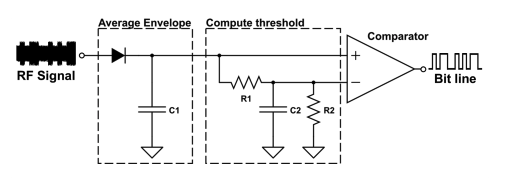
\includegraphics[scale=0.5]{backscatter_circuit}
        \label{fig:backscatter}
    \end{figure}

    Cụ thể ở bộ giải mã trong Hình 2.4, tín hiệu tán xạ ngược đầu tiên được làm mịn bởi mạch ''Average Envelope''. Sau đó mạch ''Compute threshold'' xuất ra điện áp thấp và cao của tín
    hiệu được làm mịn. Sau đó bộ so sánh ''Comparator'' so sánh tín hiệu với các ngưỡng được xác định trước để lấy ra các bit 0, 1 một cách chính xác.

\end{enumerate}

\section{Thu hoạch năng lượng.}


\section{Học tăng cường.}
\subsection{Giới thiệu.}
Học tăng cường là quá trình học xem nên làm gì, là quá trình học để kết nối giữa trạng thái và hành động nhằm mục đích tối đa hoá một giá trị phần thưởng số học. Đối tượng học sẽ không được chỉ cụ thể là
nên thực hiện hành động nào, thay vào đó phải tự mình khám phá những hành động nào mạng lại phần thưởng cao nhất bằng cách thử chúng. Hành động của đối tượng không chỉ mang lại phần thưởng ngay lập tức mà còn ảnh hưởng
đến những trạng thái tiếp theo, dẫn đến những phần thưởng tiếp theo. Hai đặc tính thử-sai và những giá trị phần thưởng đến sau là hai đặc điểm nổi bật nhất của học tăng cường.

\subsection{Quá trình ra quyết định Markov - MDP.}
Quá trình ra quyết định Markov là một khuôn khổ toán học quan trọng để mô hình hoá việc ra quyết định trong các tình huống mà kết quả một phần là ngẫu nhiên và một phần dưới sự kiểm soát
của người ra quyết định. MDP là mô tả cho một môi trường được quan sát đầy đủ cho việc học tăng cường.


\section{Học sâu tăng cường.}
\section{Mạng sâu Q - DQN.}

% Chapter 3
\chapter{Đề xuất phương pháp giải quyết bài toán gây nhiễu từ UAV.}
Trong chương này, em đề xuất phương pháp giải quyết chống nhiễu từ UAV đối với kênh truyền gồm một máy phát và một máy thu sử dụng thuật toán học tăng cường Q-learning và DQN.


\section{Mô hình hệ thống.}
Ở đây, chúng ta xem xét một hệ thống truyền thông không dây bao gồm một máy phát, một máy thu và một UAV gây nhiễu. Máy phát được trang bị bộ đệm dữ liệu để đóng vai trò như hàng đợi dữ 
liệu trước khi truyền đến máy thu, ngoài ra máy phát còn được trang bị bộ thu năng lượng và một mạch tán xạ ngược môi trường có khả năng tán xạ sóng nhiễu để truyền gói tin. Khi bị nhiễu
tấn công, máy phát có thể thu năng lượng từ tín hiệu nhiễu để sử dụng cho mục đích truyền gói tin chủ
động đến máy thu sau này khi máy gây nhiễu không tấn công - chế độ HTT, hoặc tán xạ ngược dữ liệu dựa trên sóng nhiễu - chế độ tán xạ ngược.

\begin{figure}{Mô hình hệ thống.}
    \centering
    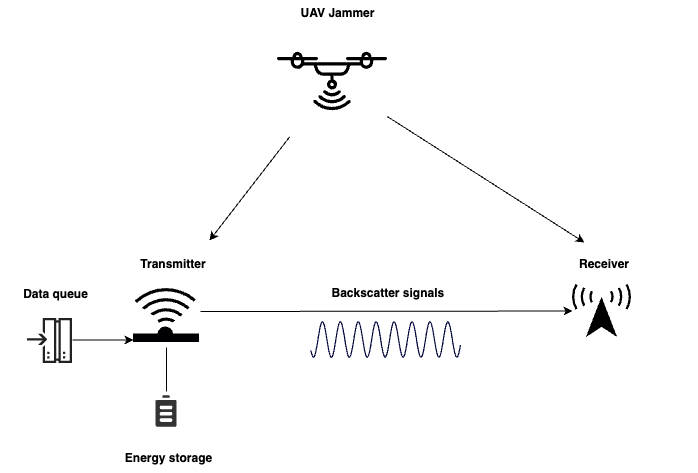
\includegraphics[scale=0.5]{system_model}
    \label{fig:system_model}
\end{figure}

\subsection{Mô hình gây nhiễu.}
Chúng ta xem xét một UAV có khả năng gây nhiễu thông minh. Giả sử UAV có khả năng lắng nghe kênh truyền giữa máy phát và máy thu khi tấn công. Điều này cho phép UAV có thể điều chỉnh vị trí
cũng như chiến lược gây nhiễu để tối đa hoá thiệt hại lên kênh truyền giữa máy phát và máy thu. Mục tiêu của UAV là làm giảm giá trị SINR tại máy thu, khiến cho kênh thông lượng của kênh
truyền giảm xuống, giá trị SINR được tính như đã trình bày ở phần cơ sở lý thuyết như sau:
\[
\theta = \frac{P_R}{\varphi P_J + \rho^2}
\]
Trong đó $P_R$ là công suất nhận được từ máy phát tại cổng (máy thu), $P_J$ là công suất nhiễu được phát của máy gây nhiễu, $\rho^2$ là phương sai của nhiễu Gauss trắng cộng thêm. 
$\varphi P_J$ là công suất nhiễu tại cổng, trong đó $0 \leq \varphi \leq 1$ là hệ số suy giảm kênh truyền.

Giá trị công suất sóng nhiễu $P_J$ của UAV tác động lên máy thu là giá trị thay đổi do UAV có khả năng thay đổi vị trí để tối ưu hoá khả năng tấn công kênh truyền như giả thiết ở trên.
Khi UAV đến gần máy phát và máy thu, khả năng xuất hiện đường truyền LoS tăng lên do góc nâng $\theta_i$
tăng lên, dẫn đến cường độ nhiễu tác động lên máy phát và máy thu tăng lên. Ngược lại khi UAV di chuyển ra xa máy phát và máy thu, khả năng gặp vật cản và các yếu tố như tăng khả năng kênh
truyền NLoS, dẫn đến cường độ nhiễu tác động lên máy phát và máy thu giảm. Ngoài ra, sẽ có những thời điểm sóng nhiễu từ UAV không tác động đến máy phát và máy thu, do sóng nhiễu có thể không
truyền đến được máy phát và máy thu do yếu tố vật cản từ môi trường, hoặc do UAV là thiết bị hạn chế về mặt năng lượng, nên có những thời điểm nó cần quay lại trạm để thay pin để bổ sung năng
lượng, khi đó UAV không tấn công kênh truyền hay cường độ gây nhiễu của UAV lên máy phát và máy thu là 0W.

Ta giả sử $P_J = \{P_0^J, \dots, P_n^J, \dots, P_N^J\}$ là vector tập các giá trị cường độ nhiễu khác nhau trong các thời điểm khác nhau của UAV. Tại mỗi thời điểm, do sự thay đổi vị trí
hoặc do yếu tố môi trường\dots, cường độ nhiễu từ UAV là khác nhau và là một trong những giá trị trong vector $P_J$ với giá trị xác suất là $x_n$. Trong đó giá trị nhỏ nhất trong vector $P_J$
là 0W, tương ứng với những thời điểm sóng nhiễu từ UAV không tác động đến kênh truyền như đã trình bày ở trên.

Ta kí hiệu $J_s = \{x = (x_0, \dots, x_n\dots, x_N), \sum_{i=0}^{N}x_n = 1\}$ là vector xác suất tấn công của UAV tương ứng với các mức năng lượng trong vector $P_J$, hay $J_s$ còn được coi như
là chiến lược tấn công của UAV.

Do UAV là thiết bị hạn chế về mặt năng lượng, UAV xác định một chiến lược tấn công $J_s$ sao cho mức công suất nhiễu trung bình $P_\text{avg}$ phù hợp với mức năng lượng và trạng thái hiện tại của UAV.
Do giả thiết UAV gây nhiễu thông minh có khả năng lắng nghe kênh truyền, chúng ta giả sử UAV gây nhiễu sẽ nhận về một phần thưởng $w_n^J$ tương ứng với mỗi giá trị $P_n^J$ trong vector $P_J$, đại diện
cho số gói tin từ máy phát đến máy thu không thành công do tác động từ sóng nhiễu (ví dụ do không giải mã thành công tại máy thu do SINR giảm). Kí hiệu $w_J = \{w_0^J, \dots, w_n^J, \dots, w_N^J\}$
là vector phần thưởng của UAV gây nhiễu. Mục tiêu của UAV gây nhiễu được xác định như sau:
\begin{align*}
    \begin{cases}
        \underset{x}{\max} \, x w_J^\top, \\
        \sum_{n=0}^{N} x_n = 1, x_n \in [0, 1], \forall n \in \{0, \dots, N\}, \\
        x P^T \leq P_\text{avg} \\
    \end{cases}
\end{align*}

\subsection{Mô hình kênh truyền.}
Khi UAV gây nhiễu không tấn công kênh truyền, hoặc khi tín hiệu nhiễu từ UAV không tác động đến kênh truyền do vật cản, máy phát có thể phát chủ động $\hat{d}_t$
gói tin đến máy thu (sử dụng phương pháp truyền dẫn chủ động thông thường), hoặc không hoạt động. Mỗi gói tin truyền thành công cần $e_t$ đơn vị năng lượng.
Khi UAV gây nhiễu tấn công và nằm trong phạm vi ảnh hưởng đến kênh truyền, máy phát vẫn có thể hoặc phát gói tin đến máy thu bằng cách điều chỉnh tốc độ phát tương
ứng với cường độ nhiễu sử dụng kỹ thuật RA, hoặc thu năng lượng từ sóng nhiễu, hoặc tán xạ ngược tín hiệu nhiễu để truyền dữ liệu đến máy thu. Thông qua các thí nghiệm
và phân tích về các hệ thống truyền thông tán xạ ngược, có thể thấy rằng với sóng nhiễu với cường độ càng lớn, càng nhiều gói tin có thể tán xạ ngược đến máy thu, và cũng
càng nhiều năng lượng có thể thu được từ sóng nhiễu nếu máy phát hoạt động ở chế độ thu năng lượng. 

Cụ thể, trong trường hợp máy
phát chọn điều chỉnh tốc độ phát dùng kĩ thuật RA, đặt $r = \{r_1, \dots, r_m,\dots, r_M\}$ là tập hợp các tốc độ truyền mà máy thu có thể lựa chọn để truyền khi bị tấn
công. Ở mỗi tốc độ $r_m$, máy phát có thể truyền tối đa $\hat{d_m^t}$ gói tin. Với $m = 1, \dots, M$ khi $\gamma_{m-1} \leq \theta < \gamma_m$ với $\gamma_m$ là giá
trị của SINR, máy thu chỉ có thể giải mã những gói tin được gửi ở tốc độ $r_0, r_1, \dots, r_\text{m-1}$, những gói tin gửi ở tốc độ $r_m$ hoặc cao hơn sẽ bị mất,
do máy thu không giải mã được. 

Trong trường hợp máy thu chọn thu năng lượng từ sóng nhiễu, năng lượng này có thể được sử dụng cho quá trình truyền chủ động sau này, tương ứng với mỗi mức cường độ nhiễu $P_n^J$
ảnh hưởng đến máy phát khác nhau, máy phát có thể thu được $e_n^J$ đơn vị năng lượng. Kí hiệu $e = \{e_0^J, \dots, e_N^J\}$ là các giá trị năng lượng có thể thu được tương ứng
với các mức nhiễu khác nhau của UAV.

Trong trường hợp máy pháp chọn tán xạ ngược sóng nhiễu để truyền dữ liệu đến máy thu, kí hiệu $\hat{d_n^J}$ là số gói tin tối đa có thể được tán xạ ngược bởi máy phát nếu
cường độ nhiễu tương ứng là $P_n^J$. Lưu ý rằng tốc độ tán xạ ngược dữ liệu được quy định bởi mạch tán xạ ngược và không thay đổi và kí hiệu là $b^{\dagger}$. Trong mô hình đề xuất này
, chúng ta giả sử khi máy phát lựa chọn tán xạ ngược sóng nhiễu, nó có thể truyền được $b^{\dagger}$ gói tin, nếu $b^{\dagger} > \hat{d_n^J}$ thì $(b^{\dagger} - d_n^J)$ gói tin sẽ bị mất trong
quá trình tán xạ ngược dữ liệu. Kí hiệu $\hat{d} = \{\hat{d_0^J}, \dots, \hat{d_N^J}\}$ là vector thể hiện số gói tin có thể được tán xạ ngược tương ứng với cường độ nhiễu.

Chúng ta kí hiệu D và E tương ứng là kích cỡ bộ đệm dữ liệu và lượng năng lượng tối đa mà máy phát có thể lưu trữ. Quá trình gói tin đến máy phát được giả sử tuân theo phân
phối Poisson với tốc độ trung bình $\lambda$. Khi bộ đệm dữ liệu của máy phát đầy, gói tin mới đến sẽ bị loại bỏ.

Lưu ý là trong hệ thống đề xuất này, máy phát chỉ có thể xác định nó có đang bị tấn công gây nhiễu hay không mà không biết cụ thể cường độ của sóng nhiễu. Thuật toán đề xuất sử dụng học tăng 
cường sâu có khả năng học được thông tin về chiến lược tấn công của UAV, cường độ của sóng nhiễu và những khả năng liên quan, qua đó đưa ra lựa chọn
phù hợp nhằm làm tối đa thông lượng trung bình của kênh truyền.


\section{Công thức hoá vấn đề.}
Để minh hoạ cho tính động và không chắc chắn của máy gây nhiễu trên UAV, chúng ta xây dựng vấn đề tối ưu hoá của hệ thống được đề cập ở trên như một quá trình ra quyết định
Markov (MDP). Việc mô hình hoá này giúp máy thu có thể ra quyết định tối ưu nhằm tối đa hoá giá trị phần thưởng dài hạn, trong trường hợp này là giá trị thông lượng trung bình
của hệ thống truyền thông. MDP được xác định bởi một bộ $\langle S, A, r \rangle$ trong đó S là không gian trạng thái, A là không gian hành động và r là hàm giá trị phần thưởng
tức thời của hệ thống.

\subsection{Không gian trạng thái.}
Không gian trạng thái trong trường hợp này được xác định bởi ba trạng thái bao gồm trạng thái của máy gây nhiễu, trạng thái của bộ đệm dữ liệu máy phát và trạng thái của bộ lưu
trữ năng lượng của máy phát.
\[
S = \{(j, d, e) : j \in \{0, 1\}; d \in \{0, \dots, D\}; e \in \{0, \dots, E\}\}
\]

Trong đó j là trạng thái UAV gây nhiễu, với $j = 0$ nếu như UAV không tấn công hoặc $j = 1$ nếu sóng nhiễu của UAV tấn công kênh truyền, d và e tương ứng là số gói tin trong bộ
đệm và số đơn vị năng lượng trong bộ lưu trữ năng lượng của máy phát. Trạng thái của hệ thống được xác định bởi một biến tổng hợp $s = (j, d, e) \in S$.

\subsection{Không gian hành động.}
Không gian hành động bao gồm $(M+4)$ hành động mà máy phát có thể lựa chọn, bao gồm không hoạt động, truyền dữ liệu chủ động, thu thập năng lượng từ sóng nhiễu, tán xạ ngược sóng
nhiễu và điều chỉnh tốc độ phát là một trong M giá trị tốc độ của vector $r = \{r_1, \dots, r_m,\dots, r_M\}$ bằng cách sử dụng kĩ thuật RA khi sóng nhiễu từ UAV ảnh hưởng đến
kênh truyền (UAV tấn công). Do đó, không gian hành động được xác định là tập $A = \{a : a \in \{1, \dots, M+4\}\}$ trong đó:

\begin{align*}
    a &= \begin{cases}
        1, & \text{Không hoạt động,} \\
        2, & \text{Truyền dữ liệu chủ động,} \\
        3, & \text{Thu hoạch năng lượng từ sóng nhiễu,} \\
        4, & \text{Tán xạ ngược dữ liệu trên sóng nhiễu,} \\
        4 + m, & \text{Điều chỉnh tốc độ phát sang } \\
                & r_m \text{ với } m \in \{1, \ldots, M\}.
    \end{cases}
\end{align*}

\subsection{Phần thưởng tức thời.}
Trong mô hình này, phần thưởng tức thời sau khi thực hiện hành động a ở trạng thái s là số gói tin được truyền thành công đến máy thu. Do đó hàm giá
trị phần thưởng tức thời được biểu diễn như sau:

\begin{align*}
    r(s,a) &= \begin{cases}
        d_t, & (j = 0, d > 0, e \geq e_t, a = 2; 0 < d_t \leq \hat{d_t}) \\
        d_n^J, & (j = 1, d > 0, a = 4; 0 < d_n^J \leq \hat{d_n^J}) \\
        d_m^r, & (j = 1, d > 0, e \geq e_t, a = 4 + m; 0 < d_m^r \leq \hat{d_m^r}) \\
        0, & \text{Trong các trường hợp còn lại.} \\
    \end{cases}
\end{align*}

Khi UAV gây nhiễu không tấn công kênh truyền (j = 0), máy phát có dữ liệu trong bộ đệm và có đủ năng lượng trong bộ lưu trữ, lúc này nó có thể chọn phát
chủ động gói tin đến máy thu (a = 2), số gói tin có thể truyền đến máy thu là $d_t$ gói tin thoả mãn $0 < d_t \leq \hat{d_t}$ gói tin.

Khi máy gây nhiễu tấn công kênh truyền (j = 1), máy phát có gói tin trong bộ đệm $(d > 0)$, nó có thể tán xạ ngược sóng nhiễu để truyền dữ liệu đến máy thu (a = 4), 
số gói tin tán xạ ngược thành công là $d_n^J$ gói tin trong đó $0 < d_n^J \leq \hat{d_n^J}$.

Ngoài ra khi máy gây nhiễu tấn công (j = 1), máy phát có gói tin trong bộ đệm $(d > 0)$ và có đủ năng lượng $(e \geq e_t)$, nó còn có thể lựa chọn phát gói 
tin với tốc độ $r_m$, (a = 4 + m) để truyển chủ động gói tin theo kĩ thuật RA, số gói tin truyền thành công đến máy thu là $d_m^r$ trong đó $0 < d_m^r \leq \hat{d_m^r}$.

Trong các trường hợp còn lại, khi máy phát không truyền thành công gói tin đến máy thu thì giá trị phần thưởng tức thời là 0.


\subsection{Công thức tối ưu hoá.}
Mục tiêu của chúng ta là tìm ra một chính sách tối ưu cho máy phát, được kí hiệu là $\pi^*$, nhằm làm tối đa hoá giá trị thông lượng trung bình
của hệ thống. Cụ thể $\pi^*$ là ánh xạ từ một trạng thái nhất định của hệ thống (trạng thái nhiễu, trạng thái bộ đệm dữ liệu và trạng thái năng
lượng của máy phát) đến một hành động tối ưu ở trạng thái đó.
Công thức hàm tối ưu hoá được xác định như sau:
\[
\max_{\pi} R(\pi) = \lim_{T \to \infty} \frac{1}{T} \sum_{k=1}^{T} \mathbb{E}\left( r_k(s_k, \pi(s_k)) \right)
\]

Trong đó $R(\pi)$ là giá trị thông lượng trung bình của máy phát tuân theo $\pi$.

$r_k(s_k, \pi(s_k))$ là giá trị phần thưởng tức thời ở thời điểm $k$ sau khi thực hiện hành động $a_k$ ở trạng thái $s_k$. 

$\pi(s_k)$ là hành động $a_k$ tuân theo chính sách $\pi$, ta thấy $\pi(s_k) = a_k$.

\section{Áp dụng phương pháp học tăng cường và học tăng cường sâu DQN để chống nhiễu.}


% Chapter 4
\chapter{Thiết lập mô phỏng và đánh giá hiệu năng.}
\section{Thông số cài đặt thử nghiệm.}
\subsection{Thông số hệ thống.}
Trong hệ thống đang được xem xét, máy phát có thể lưu trữ tối đa $D = 10$ gói tin trong hàng đợi dữ liệu, tối đa $E = 10$ đơn vị năng lượng
trong bộ lưu trữ năng lượng. Dữ liệu đến máy phát giả định tuân theo phân phối Poisson với tốc độ trung bình $\lambda = 3$ 
gói tin. Khi UAV gây nhiễu không tấn công, máy phát có thể truyền chủ động tối đa $\hat{d}_t = 4$ gói tin đến máy thu. Mỗi gói tin truyền đi cần
$e_t = 1$ đơn vị năng lượng. Do sự thay đổi vị trí của UAV như đã nói ở trên, công suất gây nhiễu của UAV cũng thay đổi, giả định tín hiệu nhiễu từ 
UAV ảnh hưởng đến đường truyền không dây đang xét gồm bốn mức $P_J = \{0W, 5W, 10W, 15W\}$ với $P_{\text{max}} = 15W$. Do lượng năng lượng
thu hoạch được cũng như số gói tin tán xạ ngược thành công tăng lên khi tín hiệu nhiễu mạnh hơn, chúng ta đặt $e = \{0, 1, 2, 3\}$ là số đơn vị
năng lượng mà máy thu có thể thu được và $\hat{d} = \{0, 1, 2, 3\}$ là số gói tin mà máy thu có thể tán xạ ngược tương ứng với mức công suất nhiễu
ảnh hưởng tới đường truyền. Ngoài ra, khi UAV tấn công gây nhiễu và máy phát sử dụng kỹ thuật RA, nó có thể truyền $d^r_m = \{2, 1, 0\}$ gói tin
tương ứng với cường độ tín hiệu nhiễu từ UAV $P^J_n = \{5W, 10W, 15W\}$. Công suất nhiễu trung bình của UAV là $P_\text{avg} = 7W$.

\subsection{Thông số cài đặt thuật toán Q-learning và DQN.}


\section{Kết quả mô phỏng.}
\subsection{So sánh sự hội tụ của hai thuật toán học tăng cường Q và DQN.}
Trong Hình 4.1, chúng ta thực hiện so sánh quá trình học để tiến đến trạng thái hội tụ của hai phương pháp DQN và Q-learning trong bài toán
chống nhiễu với các thông số môi trường như trên. Ta có thể thấy tốc độ hội tụ của thuật toán DQN là nhanh hơn so với thuật toán Q-learning.
Thậm chí sau $10^6$ lần lặp, thuật toán Q-learning vẫn chưa đạt đến trạng thái hội tụ tối ưu. Điều này là do DQN với việc sử dụng mạng thần
kinh sâu, kết hợp với việc học hỏi lại từ kinh nghiệm nhiều lần khiến nó có thể học chiến lược gây nhiễu hiệu quả hơn, qua đó đưa ra quyết định
tối ưu hơn.

\begin{figure}{Tỉ lệ hội tụ giữa DQN và Q learning.}
    \centering
    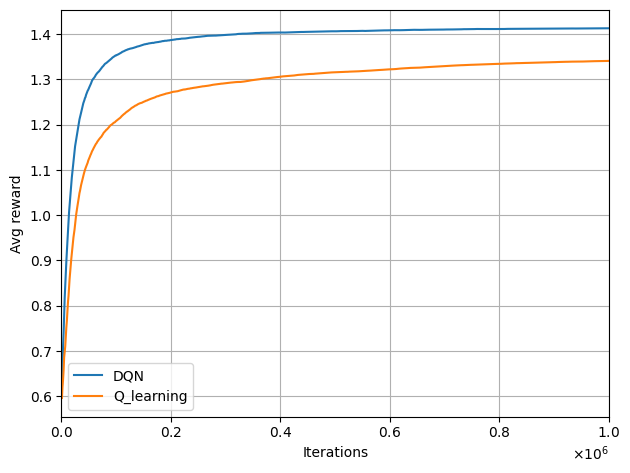
\includegraphics[scale=0.5]{converged}
    \label{fig:converged}
\end{figure}

\subsection{So sánh với chiến lược phòng thủ ''tham lam'' không sử dụng DRL.}
Ở đây, chúng ta thực hiện so sánh giữa việc sử dụng phương án DQN được đề xuất và chiến lược phòng thủ cố định ''tham lam'' được mô tả như sau: (i) Khi
UAV gây nhiễu không tấn công kênh truyền, máy phát sẽ phát chủ động gói tin đến máy thu, (ii) Khi UAV gây nhiễu tấn công kênh truyền, máy phát sẽ tận dụng
sóng nhiễu từ UAV để thu năng lượng hoặc tán xạ ngược đan xen nhau theo một chu kì cố định - máy phát sẽ tiến hành thu năng lượng từ sóng nhiễu sau mỗi chu kì
$T_\text{harvest} = 5$ đơn vị thời gian, thời gian còn lại máy phát sẽ tiến hành tán xạ ngược sóng nhiễu để truyền dữ liệu đến máy thu. Ta gọi chiến lược này
là chiến lược phòng thủ cố định ''tham lam''. Với phương án sử dụng DQN được đề xuất, em thực hiện $4 \times 10^4$ lần lặp để tìm ra chiến lược tối ưu cho máy
phát và sau đó so sánh hiệu quả với chiến lược tham lam đã nêu ở trên.

\begin{enumerate}
    \item[\textbf{a}.] \textbf{Đánh giá hiệu quả khi thay đổi công suất nhiễu.}
    \begin{figure}{So sánh thông lượng trung bình giữa DQN và Greedy $P_\text{avg}$ thay đổi.}
        \centering
        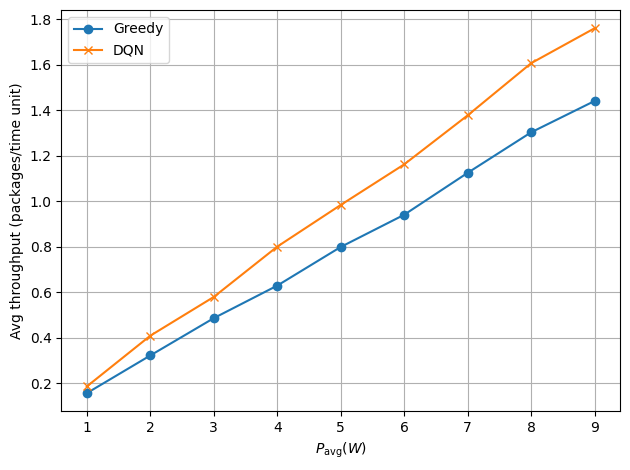
\includegraphics[scale=0.5]{p_avg_throughput}
        \label{fig:p_avg_throughput}
    \end{figure}
    \begin{figure}{So sánh số gói tin mất mát giữa DQN và Greedy $P_\text{avg}$ thay đổi.}
        \centering
        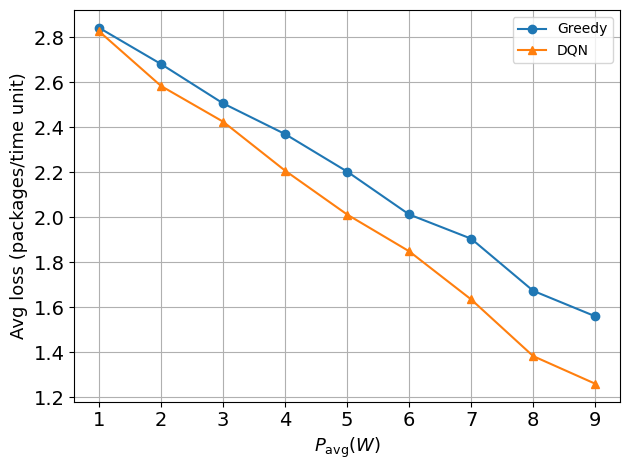
\includegraphics[scale=0.5]{p_avg_loss}
        \label{fig:p_avg_loss}
    \end{figure}
    \begin{figure}{So sánh PDR giữa DQN và Greedy $P_\text{avg}$ thay đổi.}
        \centering
        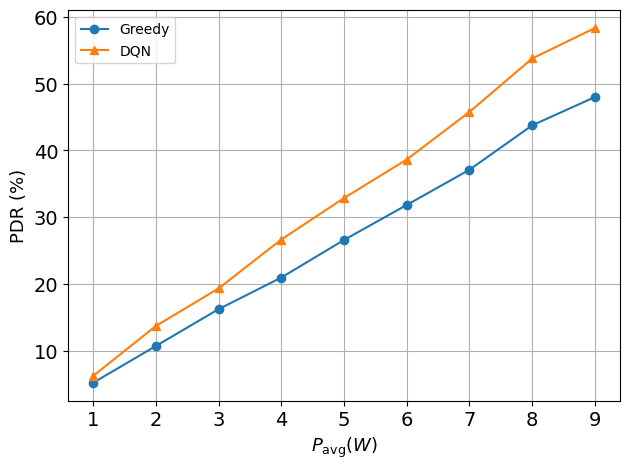
\includegraphics[scale=0.5]{p_avg_pdr}
        \label{fig:p_avg_pdr}
    \end{figure}

    Trong Hình 4.2, Hình 4.3, Hình 4.4, ta thực hiện thay đổi công suất phát của máy gây nhiễu, dễ nhận thấy khi công suất gây nhiễu tăng lên, tức là khả năng 
    máy gây nhiễu tấn công kênh truyền với mức năng lượng lớn dẫn đến khả năng tán xạ ngược sóng nhiễu và khả năng thu năng lượng từ sóng nhiễu cũng tăng lên ở 
    cả 2 phương án. Điều này đã làm cải thiện hiệu năng của hệ thống (thông lượng tăng, số gói tin mất mát giảm và tỉ lệ truyền thành công cao hơn). Tuy nhiên 
    với phương án đề xuất sử dụng học tăng cường sâu, đã giúp máy thu thích ứng được với sự bất định của môi trường nhiễu, với chiến lược tấn công dẫn đến tốc độ 
    cải thiện hiệu năng hệ thống của phương án đề xuất là cao hơn so với phương án sử dụng chiến lược “tham lam” cố định ở trên. Khi công suất trung bình của máy 
    gây nhiễu thấp, dễ nhận thấy 2 phương án có hiệu suất khá tương đồng, tuy nhiên khi công suất nhiễu trung bình càng tăng lên, sự hiệu quả của phương án đề xuất 
    càng thấy rõ.

    \item[\textbf{b}.] \textbf{Đánh giá hiệu quả khi thay đổi số gói tin có thể phát chủ động $\hat{d}_t$.}
    
    Thử nghiệm được thực hiện với công suất nhiễu $P_\text{avg} = 7W$, trong thử nghiệm ở Hình 4.5, Hình 4.6, Hình 4.7 này ta thực hiện thay đổi số gói tin tối đa mà máy phát
    có thể phát chủ động đến máy thu.

    \begin{figure}{So sánh thông lượng trung bình giữa DQN và Greedy $\hat{d}_t$ thay đổi.}
        \centering
        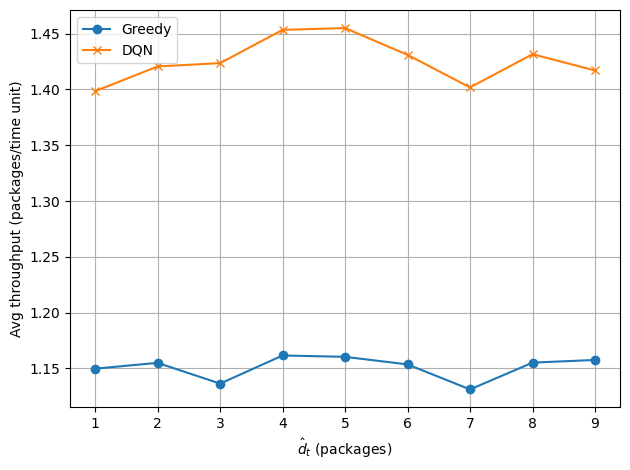
\includegraphics[scale=0.5]{dt_throughput}
        \label{fig:dt_throughput}
    \end{figure}
    \begin{figure}{So sánh số gói tin mất mát giữa DQN và Greedy $\hat{d}_t$ thay đổi.}
        \centering
        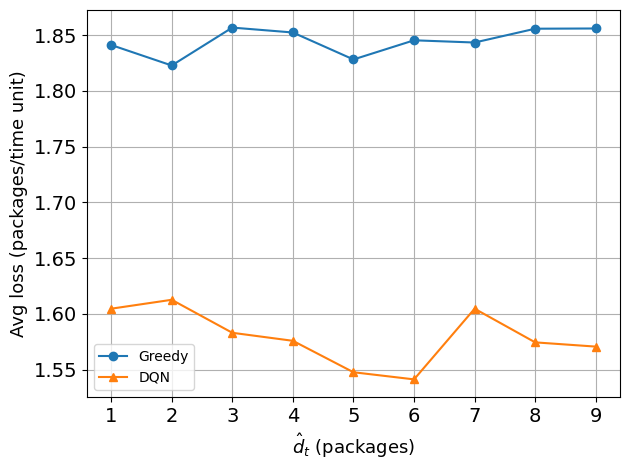
\includegraphics[scale=0.5]{dt_loss}
        \label{fig:dt_loss}
    \end{figure}
    \begin{figure}{So sánh PDR giữa DQN và Greedy $\hat{d}_t$ thay đổi.}
        \centering
        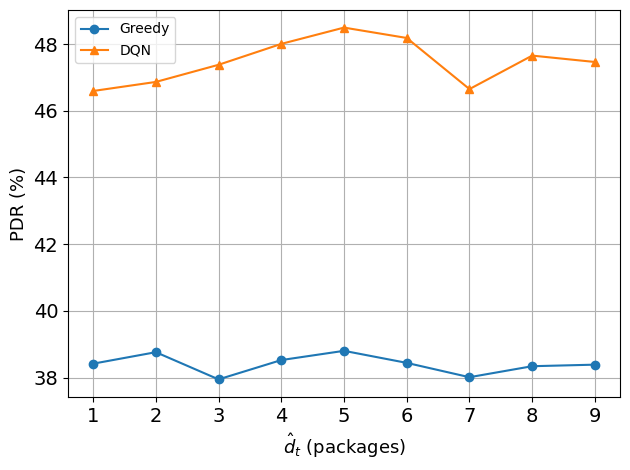
\includegraphics[scale=0.5]{dt_pdr}
        \label{fig:dt_pdr}
    \end{figure}

    \item[\textbf{c}.] \textbf{Đánh giá hiệu quả khi thay đổi chu kì thu năng lượng $T_\text{harvest}$ của máy thu trong phương án sử dụng chiến lược phòng thủ cố định “tham lam”.}
    
    Trong mô phỏng Hình 4.8, Hình 4.9, Hình 4.10 , công suất nhiễu trung bình trong mô phỏng này $P_\text{avg} = 7W$, ta thấy được việc thay đổi chu kì thu năng lượng trong 
    phương án phòng thủ tham lam khiến cho hiệu suất hệ thống thay đổi rõ rệt. Dễ thấy trong trường hợp này,  khi công suất nhiễu cao, cơ hội để máy phát có thể phát 
    chủ động không nhiều dẫn đến chiến lược phòng thủ “tham lam” chủ yếu sẽ truyền gói tin thông qua kĩ thuật tán xạ ngược, điều này khiến cho nếu chu kì thu năng lượng 
    của chiến lược “tham lam” càng lớn (càng ít thực hiện thu năng lượng hơn) sẽ khiến cho thông lượng, số gói tin bị mất và tỉ lệ gói tin thành công tăng nhanh, tuy nhiên
    khi chu kì thu năng lượng tăng đến giá trị 5 đơn vị thời gian thì hiệu quả của hệ thống với chiến lược tham lam gần như không thay đổi nhiều, do lúc này máy phát chủ yếu 
    lựa chọn tán xạ ngược thay vì thu năng lượng để chờ cơ hội phát chủ động, dẫn đến hiệu quả tán xạ ngược đã đạt gần giá trị tối ưu, khiến cho hiệu quả của hệ thống gần 
    như ổn định. Tuy nhiên vẫn chưa thể đạt đến hiệu quả như phương án đề xuất sử dụng DQN mang lại.
    \begin{figure}{So sánh thông lượng trung bình giữa DQN và Greedy $T_\text{harvest}$ thay đổi.}
        \centering
        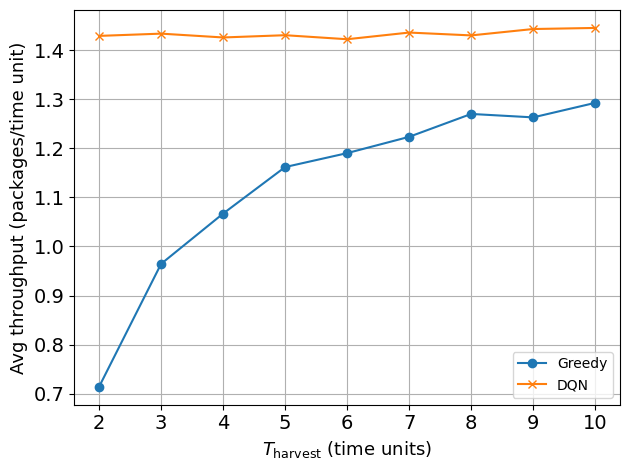
\includegraphics[scale=0.5]{t_harvest_throughput.png}
        \label{fig:t_throughput}
    \end{figure}
    \begin{figure}{So sánh số gói tin mất mát giữa DQN và Greedy $T_\text{harvest}$ thay đổi.}
        \centering
        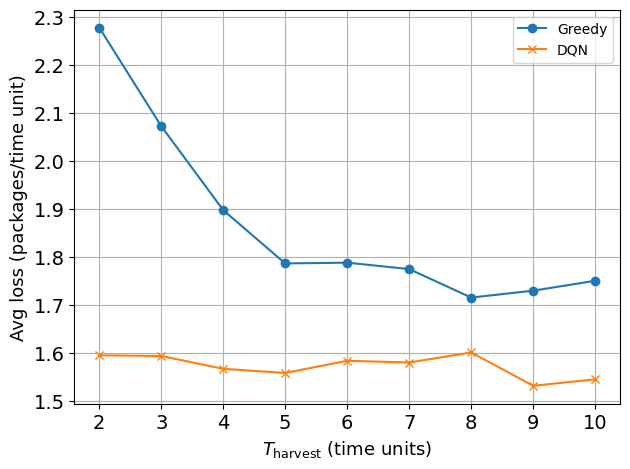
\includegraphics[scale=0.5]{t_harvest_loss.png}
        \label{fig:t_loss}
    \end{figure}
    \begin{figure}{So sánh PDR giữa DQN và Greedy $T_\text{harvest}$ thay đổi.}
        \centering
        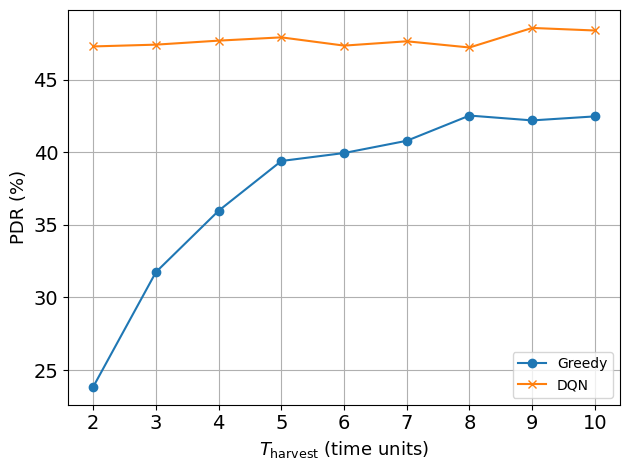
\includegraphics[scale=0.5]{t_harvest_pdr.png}
        \label{fig:t_pdr}
    \end{figure}


\end{enumerate}
% Chapter 5
\chapter{Kết luận}

% Tài liệu tham khảo
\begin{thebibliography}{9}
\begin{bibsection}{Tiếng Anh}
    % Book
    \bibitem{hoang2023deep}
    Hoang, D.T. and Van Huynh, N. and Nguyen, D.N. and Hossain, E. and Niyato, D.
    \textit{Deep Reinforcement Learning for Wireless Communications and Networking: Theory, Applications and Implementation},
    \textit{Wiley}, 2023, pp. 37-163.
    % Paper
    \bibitem{Hossein22}
    Pirayesh, Hossein and Zeng, Huacheng
    ''Jamming Attacks and Anti-Jamming Strategies in Wireless Networks: A Comprehensive Survey'',
    \textit{IEEE Communications Surveys \& Tutorials},
    vol. 24, no. 2,
    pp. 767-809

    \bibitem{Vadlamani16}
    Satish Vadlamani,Burak Eksioglu,Hugh Medal,Apurba Nandi
    ''Jamming attacks on wireless networks: A taxonomic survey'',
    \textit{International Journal of Production Economics},
    vol. 172,
    2016,
    pp. 76-94

    \bibitem{Xu2005}
    Xu, Wenyuan and Trappe, Wade and Zhang, Yanyong and Wood, Timothy
    ''The feasibility of launching and detecting jamming attacks in wireless networks'',
    \textit{Association for Computing Machinery},
    2005,
    pp. 46–57
    \bibitem{Vincent}
    Ambient Backscatter: Wireless Communication Out of Thin Air
    \bibitem{Ning_Gao}
    Anti-Intelligent UAV Jamming Strategy via Deep Q-Networks
    \bibitem{jam_me}
    “Jam Me If You Can”: Defeating Jammer with Deep Dueling Neural Network Architecture and Ambient Backscattering Augmented Communications
\end{bibsection}
\end{thebibliography}
\end{document}